\section{Literature Review}
\label{Chap2}
Before influential research in the context of \ac{SC} is presented, we want to introduce a standardized notation. Therefore, without loss of generality, assume that panel data is observed for $j = 0,1,...,J$ panel units and the unit $j = 0$ is exposed to treatment at period $T_0$. The temporal ordering is as follows:
$$
\underbrace{1,2,..., T_0 -1}_{T_{pre}},  \underbrace{T_0, T_0 +1, ..., T}_{T_{post}},
$$
such that $T_0 -1$ periods of pre-treatment data ($T_{pre}$) and $T-(T_0 -1)$ periods of post-treatment data ($T_{post}$) is observed.

\textit{Canonical Applications}\\
In their canonical 2003 article, Abadie and Gardeazabal evaluate the causal economic effects of conflict using terrorist conflicts in the Basque Country as a comparative case study. Their data consists of $T_{pre} = 15$ $(1955-1969)$ periods of pre-treatment and $T_{post} = 28$  $(1970-1997)$ periods of post-treatment data for $J = 16$ controls and the single treatment unit indexed by $j = 0$. By constructing a synthesized Basque country that is computed as a weighted average of  the remaining regions in Spain that did not experience terrorist conflicts, they invent the \ac{SC}-method to conduct causal inference in observational settings. The weights are computed such that they optimally match the central variable of interest (\ac{GDP} per capita) as well as a set of covariates of that variable for the treatment unit in the pre-treatment period. Constraining the weights to be weakly positive and to sum up to one provides an easy-to-interpret percentage interpretation and ensures that the synthetic controls generalizes in the post-treatment period. They find that terrorist conflicts caused the per capita \ac{GDP} of the treatment unit (Basque Country) to decline by about 10\% relative to the synthesized control unit. \\
The estimation of a comprehensive anti-smoking legislation in California in 1988 constituted another central application of the \ac{SC} method by \cite{abadie:2010}. Here, the outcome of interest is per capita smoking in California and 29 U.S. states without such tobacco control programs serve as control units, referred to as Donors. The authors build their estimation on only $T_{pre} = 18$ $(1970-1987)$ pre-treatment years of data and $T_{post} = 13$ $(1988-2000)$, indicating the necessity to employ alternatives to the inestimable \ac{OLS} estimator. \cite{abadie:2010} reckon that Proposition 99 had a substantial, time-increasing negative effect on per capita cigarette sales by an average of almost 20 packs per person (approximate decline of 25\%). Besides presenting the causal treatment effect, the scholars also investigate the statistical significance of their results. By applying a version of the Exact Hypothesis Test proposed by \cite{fisher:1971}, they find that the probability of experiencing a treatment effect as extreme as observed for California is only 2.6\%.\\
The reunification of East and West Germany correlated with an observable slow-down of \ac{GDP} per capita growth in West Germany. \cite{abadie:2015} utilized this natural experiment as another application of the \ac{SC}-method. In contrast to other applications of \ac{SC}, the reunification-dataset is somewhat more wealthy as data is observed for $T_{pre} = 30$ $(1960-1989)$, $T_{post} = 14$ $(1990-2003)$ years and $J = 16$ donors and West Germany. From 1992 onward, they identify a clear negative average treatment effect of about \$1,600 per capita and year (approximately 8\% reduction compared to the 1990 baseline level). In order to examine the trade-off between interpretation and statistical optimality, they sequentially remove donor units from the synthetic control and re-estimate the model. In doing so, they find that the synthetic control heavily relies on one donor (Austria), a peculiarity arising from the specific restrictions (no intercept and percent-like coefficients) of the method.

\textit{Further Applications}\\
The \ac{SC}-method is also widely used in contemporary research: For example, \cite{born:2019} apply the method to quantify the economic cost of nationalism in context of the Brexit referendum vote and find that the so-called "doppelganger gap", i.e. the difference between actual and synthesized \ac{GDP}-trajectory of the \ac{UK} ranged between 1.7 and 2.5\% after \ac{UK}'s citizens voted against remaining in the EU. To disentangle their estimated treatment effect, the scholars proceed in two steps: First, by disassembling \ac{GDP} into its components, they find that consumption and investment are the main drivers of the decline. Second, they estimate an expectation-adjusted \ac{VAR}-model to explicitly account for anticipation and uncertainty. \\
An incomplete list of recent \ac{SC} application also includes \cite{cho:2020} and  \cite{cunningham:2021}. Cho quantifies the impact of non-pharmaceutical interventions during the COVID-19 outbreak in Sweden and obtains robust indications for the adverse public health effects of tentative policy intervention during the COVID-19 pandemic. Cunningham studies the effect of incarceration in Texas to drug markets. Besides identifying only moderate effects of Texas doubling the state's prison capacities on the drug market, Cunningham has a salient point on the practical use of \ac{SC}: "Authors using synthetic control must do more than merely run the synth command when doing comparative case studies. They must find the exact p-values through placebo-based inference, check for the quality of the pre-treatment fit, investigate the balance of the covariates used for matching, and check for the validity of the model through placebo estimation [...]."

\textit{Developments}\\
\cite{athey:2016} examine the topic of causal inference in observational studies at a higher level of abstraction and present their often quoted assessment of \ac{SC} being arguable "the most important innovation in policy innovation in the last 15 years". \\
\cite{doudchenko:2016} specifically focus on the identifying assumptions of \ac{SC}. Besides the careful treatment of the relationship between the amount of explanatory variables $J$ and pre-treatment observations $T_{pre}$, they elaborate in great detail on the four prevailing restrictions on the intercept and the weights, namely the no-intercept assumption, adding-up and non-negativity as well as the potential assumption of constant weights. Their main recommendation is to leave the restrictions aside and to opt for an elastic-net regression that ensures external validity by means of regularization. They apply the elastic together with three other proposal models to three core applications of \ac{SC} and obtain comparable results for the different models. \\
\cite{benmichael:2021a} connect to the commonly violated assumption of a perfect pre-treatment fit of the original \ac{SC} method: they introduce the augmented synthetic control method that accounts for a potential bias of the \ac{SC}-estimator due to imperfect pre-treatment fit. Simplified, their model uses a ridge penalty to improve the pre-treatment and penalizes extrapolation from the convex hull of the donors. In some applications, interventions are subject to staggered adoption, i.e. multiple panel units adopting a given given treatment at different times. \cite{benmichael:2021b} generalize the original \ac{SC}-method to such scenarios by proposing a "partially pooled" \ac{SC} that allows for unit-level intercepts and covariates.  

\cite{abadie:2019} \\
\cite{amjad:2018} \\
\cite{harvey:2020} \\
\cite{muhlbach:2019}

\textit{Hypothesis Tesing}\\
The question of treatment effect significance arises naturally subsequent to the construction of the synthetic control. \ac{ADH} propose a model-invariant non-parametric inference procedure that is based on the Exact Hypothesis Test proposed by \cite{fisher:1971}. \footnote{The basic idea behind such permutation tests is to compare the observed data with a number of randomly permuted versions of it, and to use the distribution of the test statistic calculated from the permutations to estimate the probability that the observed result occurred by chance.} 
\ac{ADH} consider permutations in region (i.e. panel unit) and time. Region permutations estimate the treatment effect for each panel unit $j \in \{0, ..., J \}$.\footnote{Note that it is necessary to exclude the truly treated unit from donor pool as otherwise, it will contaminate the synthetic control} This procedure provides the researcher with the empirical $(J+1)$-observational distribution of the treatment. Next, the estimated treatment effect of the truly treated unit can be compared to the $J$ placebo-treatment effects of the donors. Given the estimated treatment effect for the truly treated unit is large, the null hypothesis of no treatment effect can be rejected at the significance level of one minus the percentile of treatment effect in the empirical distribution.\footnote{For instance, let $J = 99$ such that treatment effects for 100 panel units can be computed. As long as the estimated treatment effect of the truly treated units belongs to the 95 most extreme effects (95th percentile or higher), the permutation test rejects the null hypothesis of no treatment effect at least at 5 percent.} Time permutations consider only the truly treated unit and permute the treatment to time periods prior to the true treatment date $T_0$. Given that $T_0 \gg J$, this approach can increase the sensitivity of the test, since the theoretically feasible significance threshold of region permutation tests is determined by $\frac{1}{J}$. For both, region and time permutations, \ac{ADH} condense the estimated treatment effects into a precision metric like the \ac{MSE}. Outlier in the donor pool can cause problems: Suppose for instance, that one donor region is very different from the rest such that it falls outside the convex hull of the remaining donors.\footnote{Note, that this circumstance does not cause problems for the truly treated region and its synthesized counterfactual as we expect the \ac{SC}-algorithm to assign a near zero weight to such an outlier. } Since the outlier itself cannot be synthesized precisely by the donor pool, pre- and post-treatment \ac{MSE} are expected to be large. Consequently, the permutation test will be unreasonably conservative and \ac{ADH} propose to exclude regions that are hard to predict, i.e. who have a pre-treatment \ac{MSE} that exceeds the \ac{MSE} of the truly treated unit to a great extent. Figure \ref{F_01} visualizes the exclusion procedure in the tobacco control application of \ac{ADH}. 

\begin{figure}[H]
	\centering
	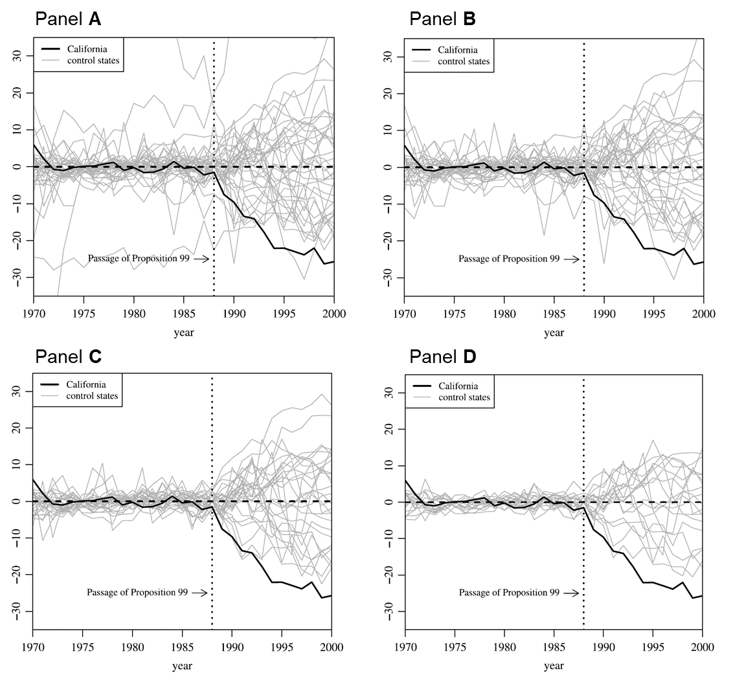
\includegraphics[scale=0.75]{F01}
	\caption{Region Exclusion Procedure of ADH}
	\label{F_01}
\end{figure}

The vertical axis indicates the gap between observed and estimated  per capita cigarette sales, the bold line represents the truly treated region (California). Some regions have both a poor pre- and post-treatment fit. Since the treatment significance should not be artificially driven by regions with poor fit, \ac{ADH} successively remove regions with a large pre-treatment \ac{MSE} relative to California. Panel B excludes regions with a \ac{MSE} that is more than 20 times as large the \ac{MSE} of California, Panel C lowers the cutoff to five times California's \ac{MSE} and Panel D to  two times the \ac{MSE}. In the last scenario, only 19 regions are left and California is the one with the most extreme treatment effect. The authors therefore conclude that the treatment is statistically significant with a (permutation) p-value of 5,3\% $\left(  \frac{1}{19} \right) $. One way to bypass the inefficient sample reduction procedure is to look at the distribution of the ratios of pre- and post-treatment \ac{MSE}. By scaling the post-treatment fit by the pre-treatment fit, regions with a poor fit are implicitly controlled for. In the tobacco control application, California is the region with the highest pre- to post-treatment \ac{MSE} ratio among all 39 regions, translating into a p-value of 2.6\% $\left(  \frac{1}{39} \right) $. 

\cite{andrews:2003} not read. \\
\cite{chernozhukov:2019} not read.\\
\cite{chernozhukov:2021} not read. \\
\cite{firpo:2018} not read. \\
\cite{hahn:2017} read.\\
\cite{breitung:2021}







